\def\mytitle{IDE ASSIGNMENT}
\def\myauthor{KALPANA}
\def\contact{kalpanamudhiraj29@gmail.com}
\def\mymodule{Future Wireless Communications (FWC)}
\documentclass[journal,12pt,twocolumn]{IEEEtran}

\usepackage{enumitem}
%\usepackage{amsmath}
\usepackage{amsfonts}
\usepackage{setspace}
\usepackage{gensymb}
\usepackage{xcolor}
\usepackage{caption}
\usepackage[hyphens,spaces,obeyspaces]{url}
\usepackage[cmex10]{amsmath}
%\usepackage{mathtools}
%\singlespacing
%\usepackage{amsthm}
%\usepackage{mathrsfs}
%\usepackage{txfonts}
%\usepackage{stfloats}
%\usepackage{cite}
%\usepackage{cases}
%\usepackage{subfig}
%\usepackage{longtable}
%\usepackage{multirow}
%\twocolumn
\usepackage{graphicx}
%\graphicspath{{./images/}}
%\usepackage[colorlinks,linkcolor={black},citecolor={blue!80!black},urlcolor={blue!80!black}]{hyperref}
%\usepackage[parfill]{parskip}
%\usepackage{lmodern}
%\usepackage{tikz}
%\usepackage{circuitikz}
%\usepackage{karnaugh-map}
%\usepackage{pgf}
%\usepackage[hyphenbreaks]{breakurl}

\usepackage{tabularx}
%\usetikzlibrary{calc}

\renewcommand*\familydefault{\sfdefault}
\usepackage{watermark}
\usepackage{lipsum}
\usepackage{xcolor}
\usepackage{listings}
\usepackage{float}
\usepackage{titlesec}
\DeclareMathOperator*{\Res}{Res}
\renewcommand\thesection{\arabic{section}}
\renewcommand\thesubsection{\thesection.\arabic{subsection}}
\renewcommand\thesubsubsection{\thesubsection.\arabic{subsubsection}}

\renewcommand\thesectiondis{\arabic{section}}
\renewcommand\thesubsectiondis{\thesectiondis.\arabic{subsection}}
\renewcommand\thesubsubsectiondis{\thesubsectiondis.\arabic{subsubsection}}
\titlespacing{\subsection}{1pt}{\parskip}{3pt}
\titlespacing{\subsubsection}{0pt}{\parskip}{-\parskip}
\titlespacing{\paragraph}{0pt}{\parskip}{\parskip}
\newcommand{\figuremacro}[5]{
    \begin{figure}[#1]
        \centering
        \includegraphics[width=#5\columnwidth]{#2}
        \caption[#3]{\textbf{#3}#4}
        \label{fig:#2}
    \end{figure}
}

\lstset{
frame=single, 
breaklines=true,
columns=fullflexible
}

%\thiswatermark{\centering \put(400,-128.0){\includegraphics[scale=0.3]{logo}} }
\title{\mytitle}
\author{\myauthor\hspace{1em}\\\contact\\IITH\hspace{0.5em}-\hspace{0.6em}\mymodule}
\date{20-12-2022}
\def\inputGnumericTable{}                                 %%
\lstset{
%language=C,
frame=single, 
breaklines=true,
columns=fullflexible
}
 \begin{document}
%

%\theoremstyle{definition}
\newtheorem{theorem}{Theorem}[section]
\newtheorem{problem}{Problem}
\newtheorem{proposition}{Proposition}[section]
\newtheorem{lemma}{Lemma}[section]
\newtheorem{corollary}[theorem]{Corollary}
\newtheorem{example}{Example}[section]
\newtheorem{definition}{Definition}[section]
%\newtheorem{algorithm}{Algorithm}[section]
%\newtheorem{cor}{Corollary}
\newcommand{\BEQA}{\begin{eqnarray}}
\newcommand{\EEQA}{\end{eqnarray}}
\newcommand{\define}{\stackrel{\triangle}{=}}
\bibliographystyle{IEEEtran}

\vspace{3cm}
\maketitle
\tableofcontents
  \section{QUESTION}
  Implementation of Seven Segment using Arduino UNO \\

     \section{COMPONENTS}
     \begin{tabularx}{0.46\textwidth} { 
  | >{\centering\arraybackslash}X 
  | >{\centering\arraybackslash}X 
  | >{\centering\arraybackslash}X
  | >{\centering\arraybackslash}X | }
\hline
\textbf{Component}& \textbf{Values} & \textbf{Quantity}\\
\hline
Arduino & UNO & 1 \\  
\hline
JumperWires & M-F & 30 \\ 
\hline
seven segment &common Anode &1\\
\hline
Bread-board & & 1\\
\hline
Resistors &220ohms &1\\

\hline
\end{tabularx}

 \begin{center}
Figure.Components
 \end{center}

\section{PIN DIAGRAM}
\begin{figure}[H]
\centering
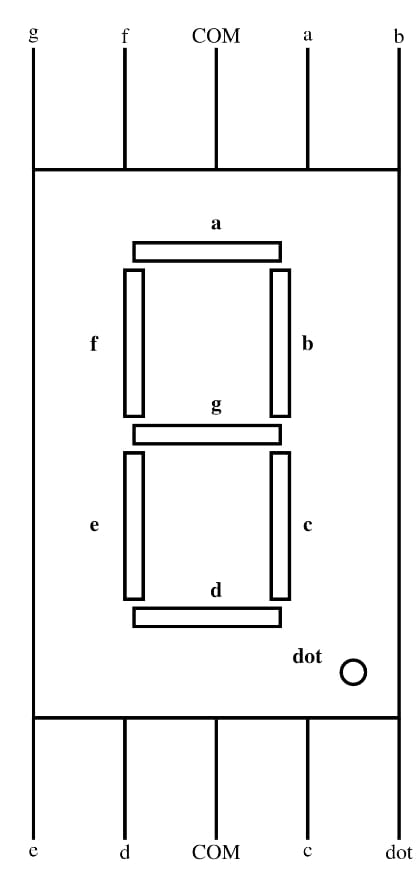
\includegraphics[width=0.4\textwidth]{pin.jpg}
\caption{Seven Segment pins}
\label{fig:div5 circuit.jpg}
\end{figure}



\section{HARDWARE}
\begin{enumerate}
\item Make the connections between the seven segment display and the Arduino as shown below.\\
	\begin{table}[h!]
    \centering
    \small  % This makes the font size smaller for the table content
    \begin{tabular}{|c|c|c|c|c|c|c|c|}
        \hline
        \textbf{Arduino}  & 2 & 3 & 4 & 5 & 6 & 7 & 8\\
        \hline
        \textbf{Display} &a&b&c&d&e&f&g\\
        \hline
    \end{tabular}
\end{table} 


\end{enumerate}7
\section{SEVEN SEGMENT OUTPUT}
\begin{figure}[H]
\centering
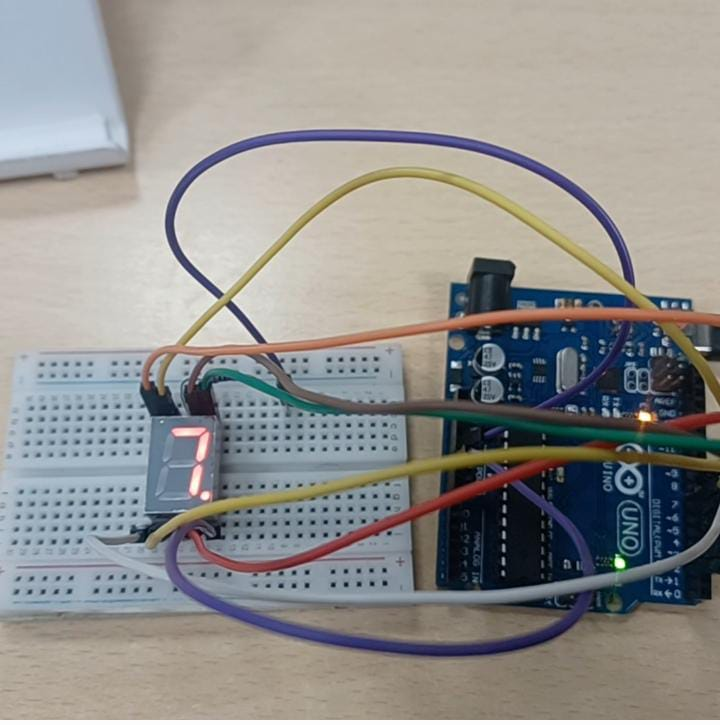
\includegraphics[width=0.4\textwidth]{1.jpg}
\caption{Connections}
\label{fig:connection.jpg}
\end{figure}

    \section{CONCLUSION}
    Hence we have implemented the Seven Segment Display using the Arduino \\
    \\
    \begin{tabularx}{0.46\textwidth} { 
  | >{\centering\arraybackslash}X |}
  \hline 
https://github.com/kalpanasunkari\\ /FWC/blob/main/Seven-segment/main.cpp\\
  \hline
\end{tabularx}

 \bibliographystyle{ieeetr}
\end{document}
